The dashboard integrates the backend processes mentioned above using FastAPI endpoints. It is important to interact with the run-time processes in a user/operator friendly manner. The dashboard consists of an argument parser console, chatbot, a network visualizer and a status bar that aids the decision making by the operator or users.

\begin{figure*}
    \centering
    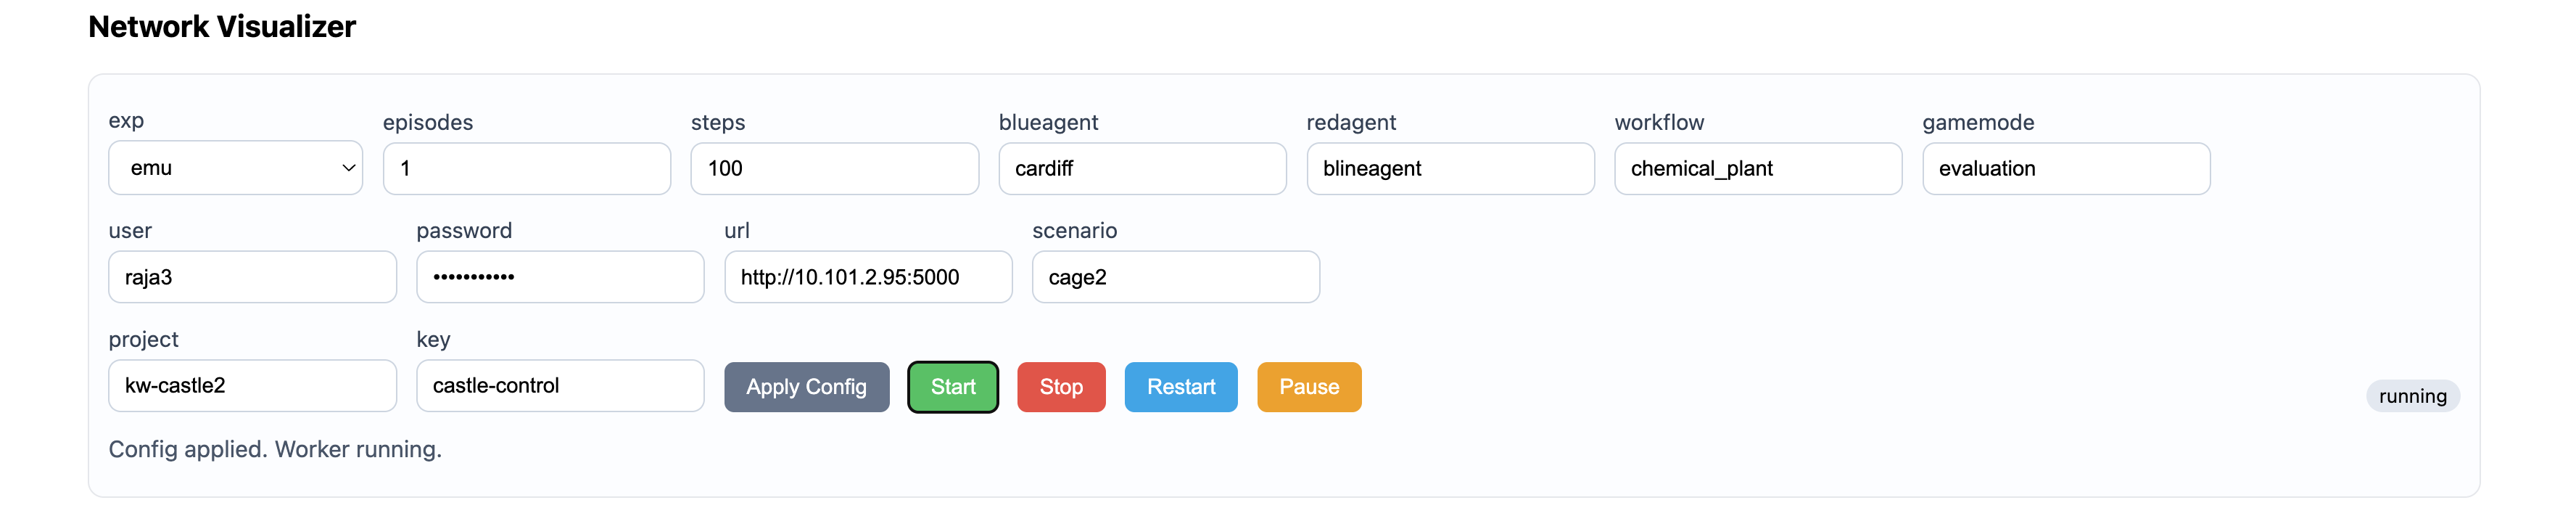
\includegraphics[width=\linewidth]{Figures/arguments.png}
    \caption{Dashboard to parse the experiment attributes.}
    \label{fig:argument_parser}
\end{figure*}

% \begin{figure*}
%     \centering
%     \includegraphics[width=\linewidth]{Figures/Network_visualizer.png}
%     \caption{Network visualizer to visualize the network topology along with red and blue attack paths.}
%     \label{fig:network_visualizer}
% \end{figure*}

% \begin{figure*}
%     \centering
%     \includegraphics[width=\linewidth]{Figures/Shap_values_actions.png}
%     \caption{Observation dashboard displaying the SHAP values and the corresponding actions.}
%     \label{fig:observation_dashboard}
% \end{figure*}

% \begin{figure*}
%     \centering
%     \includegraphics[width=\linewidth]{Figures/chat.png}
%     \caption{Chat returned by the LLM agent based on the operator query on workflow pause .}
%     \label{fig:chat_bot}
% \end{figure*}

The LLM logs (shown in Figure \ref{fig:reward_comparison}) is integrated into a browser-based operator dashboard served by a FastAPI application and accessed via a standard web interface. To enable meaningful human-in-the-loop interaction without interrupting simulation continuity, the dashboard implements a \emph{pause-and-explain} mechanism controlled by a dedicated pause toggle. When the operator activates the pause, the simulation halts at the
conclusion of the current iteration and the system enters a two-phase explanation flow. In the first phase, the dashboard immediately renders the current network state and SHAP-derived feature attributions, while displaying a visual loading indicator in place of the action selection panel; this communicates that the system is actively generating an explanation and prevents premature interaction. Concurrently, the
backend asynchronously queries the LLM with a prompt constructed from the current iteration context, including the blue and red agent actions extracted from the simulation state. In the second phase, once the LLM returns its response, the explanation text is pushed to the UI via a thread-safe snapshot bridge, the action selection panel becomes active, and the \emph{Resume} button is enabled. This sequencing ensures that operators always read the explanation before they commit to an action or continue the simulation, enforcing the intended Human-AI collaboration loop.
The synchronization between the simulation worker thread and the operator dashboard is managed through a pair of threading primitives. A \texttt{pause\_event} signals when the simulation has reached a pause point, while an \texttt{action\_selected\_event} blocks the worker until the operator has either selected an override action or clicked \emph{Resume}. A boolean flag \texttt{\_llm\_ready} gates the availability of the \emph{Resume} button in the UI, preventing the operator from advancing the simulation before the explanation has been delivered. The dashboard polls the backend at \textit{300\,ms} intervals for snapshot updates (network graph, SHAP values, available actions) and at \textit{1\,s} intervals for pause and readiness status, providing near-real-time feedback without overloading the server. Once an explanation has been displayed, it persists in the UI panel for the duration of the pause regardless of subsequent snapshot updates, so the operator can continue reading while reviewing the network visualization.

The operator action selection panel renders the set of candidate blue agent actions as clickable buttons. 
Selecting an action immediately records the operator's choice and signals the worker to resume with that action, bypassing the agent's default policy for that iteration. If no action is selected within a configurable timeout window, the simulation resumes automatically with the agent's original recommendation. 
This design preserves operational tempo while still allowing operators to intervene when the LLM explanation or SHAP attribution highlights a concern.

Together, the SHAP attributions, the decision tree policy extraction, and the LLM chatbot form a layered explanation system. SHAP values identify \emph{which features} drove the agent's decision; the decision tree renders the \emph{policy logic} in human-readable form; and the LLM chatbot translates both into \emph{natural language narrative} tailored to the operator's query. This layered approach reflects best practices in human-centered XAI, providing multiple complementary explanation modalities~\cite{ye2023complementary} while keeping the operator in meaningful control of the simulation's trajectory.
%Figure \ref{fig:argument_parser} gives quick overview of this feature.
